%!TEX root = ../Thesis.tex
\section{Sutskever}

As no neural network framework exists for creating networks like the Sutskever model, such a framework was written as a part of this thesis. This is a big task where a lot can go wrong, so the first part of this section will attempt to validate the model by having it solve some simple problems.

\subsection{Constructed problems}

Inspired from the learning to execute paper \cite{learning-to-execute} a copy problem is used to validate the model. The idea is simple, generate a sequence of random integers between 1 and 9 of length 8 and append an \texttt{<EOS>} element (encoded 0) to that sequence. 
\begin{figure}[H]
\begin{equation*}
\begin{aligned}
[3, 4, 8, 5, 9, 9, 4, 4, 0] \\
[2, 5, 9, 7, 6, 2, 1, 5, 0] \\
[1, 6, 7, 4, 4, 1, 6, 4, 0]
\end{aligned}
\end{equation*}
\caption{Example of integer sequences used in the \textit{copy} problem.}
\end{figure}

Each element of value $i$ is then transformed into an indicator vector, such that the 1-element is at position $i$. The indicator vector will be denoted by a bold font.

Now consider the following three variations of the same problem. Note that that only the \textit{full network} model is required and used for the immediate validation. But the \textit{encoder} and \textit{decoder} problems becomes useful in a detailed analysis.

\paragraph{Full network} To validate the full network the sequence of indicator vectors is used both as input and output. Example: $[\mathbf{3}, \mathbf{4}, \mathbf{8}, \mathbf{5}, \mathbf{9}, \mathbf{9}, \mathbf{4}, \mathbf{4}, \mathbf{0}] \rightarrow [\mathbf{3}, \mathbf{4}, \mathbf{8}, \mathbf{5}, \mathbf{9}, \mathbf{9}, \mathbf{4}, \mathbf{4}, \mathbf{0}]$.

\paragraph{Encoder} The encoder problem is a regression problem where the output is the integer sequence expressed as an vector. Note that the \texttt{<EOS>} isn't included and the vector is divided by 9 to fit between $0$ and $1$. It isn't strictly necessary for the output to be within $[0, 1]$, but it makes it easier to compare to the decoder version of this problem. Example: $[\mathbf{3}, \mathbf{4}, \mathbf{8}, \mathbf{5}, \mathbf{9}, \mathbf{9}, \mathbf{4}, \mathbf{4}, \mathbf{0}] \rightarrow [\sfrac{3}{9}, \sfrac{4}{9}, \sfrac{8}{9}, \sfrac{5}{9}, \sfrac{9}{9}, \sfrac{9}{9}, \sfrac{4}{9}, \sfrac{4}{9}]$.

\paragraph{Decoder} Finally one can consider a decoder version of the \textit{copy} problem. Here the input should be between $0$ and $1$, as this will be used to initialize the hidden output $b_{h_1}^{0_d}$ and the cell state $s_{h_1}^{0_d}$. The cell in partially is almost always in the $[0, 1]$ interval. The input and output is the same as in the encoder case, just swapped. Example: $[\sfrac{3}{9}, \sfrac{4}{9}, \sfrac{8}{9}, \sfrac{5}{9}, \sfrac{9}{9}, \sfrac{9}{9}, \sfrac{4}{9}, \sfrac{4}{9}] \rightarrow [\mathbf{3}, \mathbf{4}, \mathbf{8}, \mathbf{5}, \mathbf{9}, \mathbf{9}, \mathbf{4}, \mathbf{4}, \mathbf{0}]$

\subsection{Validating implementation}

To validate the Sutskever model the \textit{full network} version of the \textit{copy} problem was used. The model was configured as:

\begin{table}[H]
\centering
\begin{tabular}{r|c}
	parameter & value \\ \hline
	learning rate ($\eta$) & 0.001 \\
	momentum ($m$) & 0.9 \\
	decay ($\gamma$) & 0.95 \\
	weight initialization & $\mathcal{N}(0, 0.5^2)$ \\
	clipping strategy & Euclidean \\
	clipping value & 10
\end{tabular}
\caption{Initialization parameters.}
\end{table}

In all cases the sigmoid function was used in the gate (f) non-linear function and the input non-linear function (g). The output activation function (h) was set to the identity function. Such that the LSTM unit can generalize to the simple RNN unit.

Note also that the target value wasn't reversed, this is to make the model easier to reason about. The original paper \cite{sutskever} also indicates that the model does work without reversing the target value, it just improves the performance.

\begin{figure}[H]
	\centering
	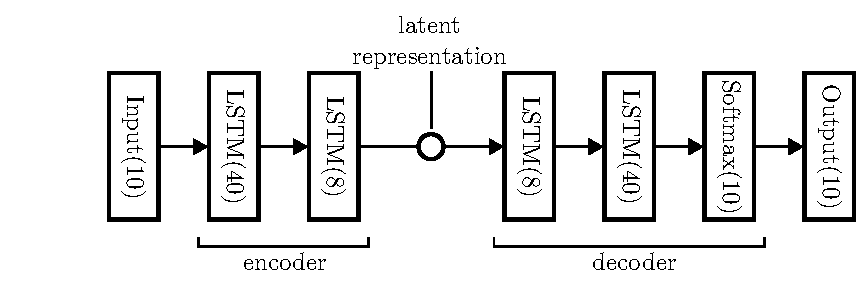
\includegraphics[scale=0.7]{results/sutskever-validate}
	\caption{The architecture of the network.}
\end{figure}

The loss curve in Figure \ref{fig:results:sutskever:network-05} shows that the implementation is capable of solving the copy problem and actually converges fairly nicely with a very minimal overfitting.

Whether or not the model solves it such that the encoder solves the \textit{encoder copy} problem and the decoder solves the \textit{decoder copy} is unknown. This is also irrelevant for validating the implementation. However the loss curves are for those two problems are still shown here in Figure \ref{fig:results:sutskever:decoder-encoder-05}, as they will later prove valuable as a reference.

Also note that while solving this problem validates the implementation, it doesn't guarantee an correct implementation, it just makes it likely that the implementation is correct.

\begin{figure}[h]
	\centering
	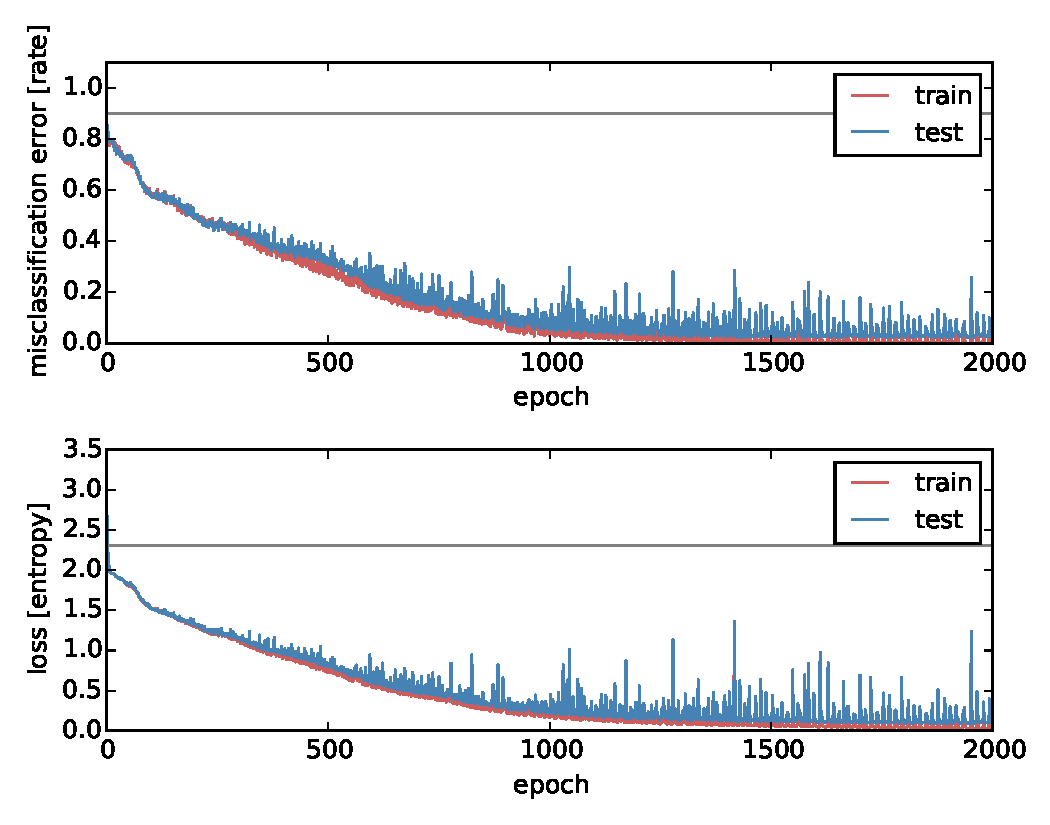
\includegraphics[scale=0.60]{results/sutskever-network-normal-05-rmsgraves}
	\caption{Loss and misclassification rate as a function of the number of epochs on the full Sutskever network.}
	\label{fig:results:sutskever:network-05}
\end{figure}
\begin{figure}[H]
        \vspace{-0.5cm}
        \centering
        \begin{subfigure}[b]{0.49\textwidth}
                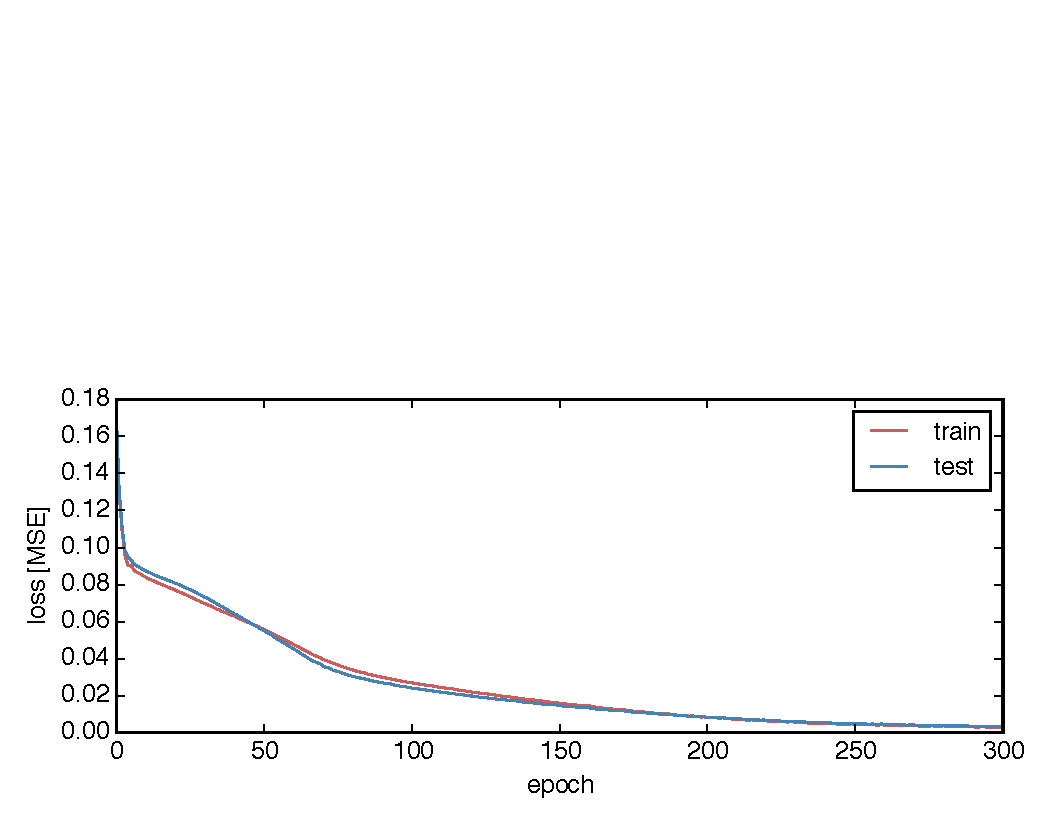
\includegraphics[scale=0.60]{results/sutskever-encoder-normal-05-rmsgraves}
                \caption{Encoder}
        \end{subfigure}
        \begin{subfigure}[b]{0.49\textwidth}
                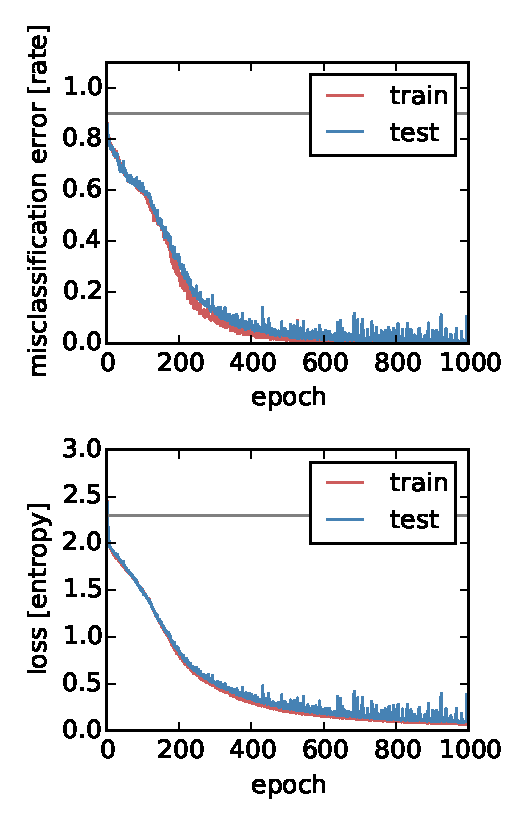
\includegraphics[scale=0.60]{results/sutskever-decoder-normal-05-rmsgraves}
                \caption{Decoder}
        \end{subfigure}
        \caption{Loss and misclassification rate as a function of the number of epochs.}
        \label{fig:results:sutskever:decoder-encoder-05}
\end{figure}

\subsection{Using real data}

Now that the implementation is validated, it can be used on the real problem. The goal is to predict the article title given the article lead. The hope is this should be somewhat similar to the translation problem solved in the original paper \cite{sutskever}. Figure \ref{fig:results:sutskever:example} shows the first 3 observations in the dataset. The entire dataset consists of 273813 news articles, all articles are used for training.

\begin{figure}[H]
\centering
\begin{tabular}{r|p{10cm}}
	title: & Ukrainian President Yanukovych agrees early election \\
	lead: & Ukrainian President Yanukovych calls an early election, as details emerge of a deal to end political crisis. Ukrainian President Viktor Yanukovych has agreed to an early presidential election as part of a deal to end the long-running crisis.
\end{tabular}
\mbox{}\vspace*{0.5cm}
\begin{tabular}{r|p{10cm}}
	title: & UK floods: Damage 'could have been prevented' \\
	lead: & Damage during the recent floods could have been prevented if the correct water management techniques had been used, says a group of experts.Some of the damage caused by the recent floods could have been prevented if the correct water management techniques had been used, says a group of leading environmental and planning experts.
\end{tabular}
\mbox{}\vspace*{0.5cm}
\begin{tabular}{r|p{10cm}}
	title: & Five lose housing benefit cut appeal \\
	lead: & Five disabled social housing tenants lose their Court of Appeal bid to have benefit cuts for those with spare bedrooms ruled unlawful. Five disabled social housing tenants have lost their Court of Appeal bid to have benefit cuts for those with spare bedrooms ruled unlawful.
\end{tabular}
\caption{Three examples on title (target) and lead (input).}
\label{fig:results:sutskever:example}
\end{figure}

It turns out that using $\mathcal{N}(0, 0.5^2)$ to initialize the weights has such a high variance that the gradients become not-a-number (NaN). To solve this $\mathcal{N}(0, 0.1^2)$ is used to initialize the weights, this is also what Alex Graves uses in his book \cite{alexgraves}.

This allows the training to continue for some iterations, to have it to continue for a longer duration with out getting not-a-number gradients the momentum and learning rate is also decreased. The final configuration is shown in Table \ref{fig:results:sutskever:article-parameters} and Figure \ref{fig:results:sutskever:article-artitecture}.
\begin{table}[h]
\centering
\begin{tabular}{r|c}
	parameter & value \\ \hline
	learning rate ($\eta$) & 0.0001 \\
	momentum ($m$) & 0.2 \\
	decay ($\gamma$) & 0.95 \\
	weight initialization & $\mathcal{N}(0, 0.1^2)$ \\
	clipping strategy & Euclidean \\
	clipping value & 10
\end{tabular}
\caption{Initialization parameters.}
\label{fig:results:sutskever:article-parameters}
\end{table}

\begin{figure}[h]
	\centering
	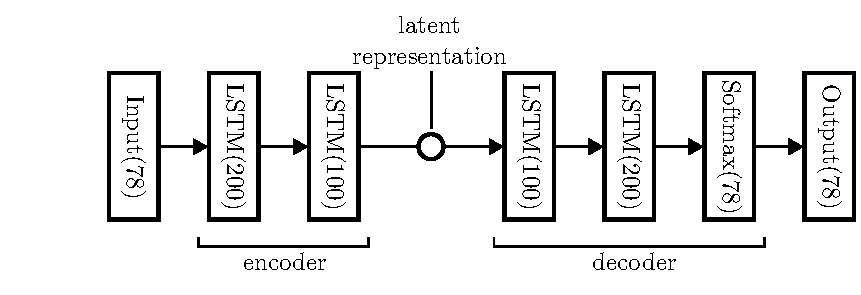
\includegraphics[scale=0.7]{results/sutskever-article}
	\caption{The architecture of the network.}
	\label{fig:results:sutskever:article-artitecture}
\end{figure}

\begin{figure}[H]
	\centering
	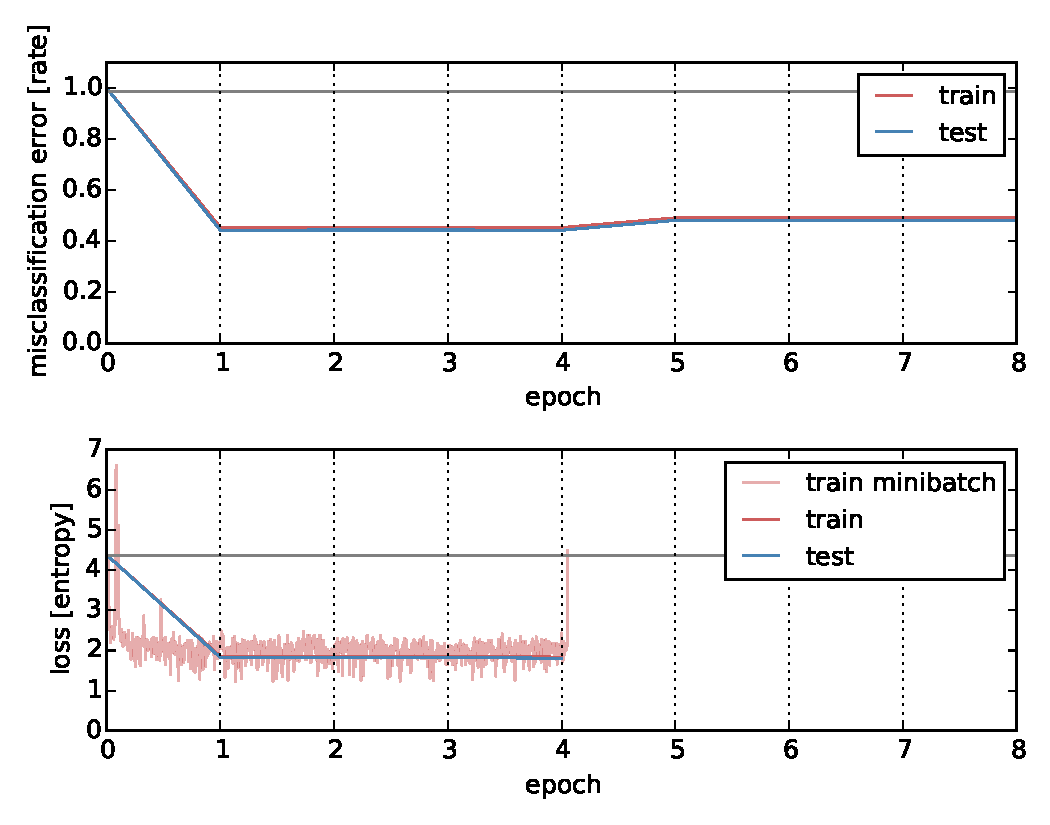
\includegraphics[scale=0.60]{results/sutskever-article-normal-01-rmsgraves-m02.pdf}
	\caption{Loss and misclassification rate as a function of the number of epochs on the full Sutskever network.}
	\label{fig:results:sutskever:article-learning}
\end{figure}

Figure \ref{fig:results:sutskever:article-learning} shows that the model didn't converge after 4 epochs. Note that after approximately 4 epochs the gradients became not-a-number. The misclassification rate is only $0.5$ so maybe there could be some meaning in the output. But from inspecting the prediction for the first 3 observations (Se Table \ref{fig:results:sutskever:predictions}) it is clear that isn't the case.
\begin{table}[h]
\centering
\begin{tabular}{p{9cm}|p{2cm}}
	target & prediction \\ \hline
	Ukrainian President Yanukovych agrees early election & \texttt{<EOS>} \\
	UK floods Damage 'could have been prevented' & \texttt{<EOS>} \\
	Five lose housing benefit cut appeal & \texttt{<EOS>}
\end{tabular}
\caption{Target and prediction of the first 3 observations.}
\label{fig:results:sutskever:predictions}
\end{table}

The model just predicts a long sequence of \texttt{<EOS>} which will match a fairly big part of the target, because the target is padded with \texttt{<EOS>} to fit the longest sequence in that mini-batch.

Each epoch contains 2140 mini-batches and takes about 3 hours to run. The 4 epochs that ran before the gradients became not-a-number thus took 12 hours. This should be enough time to find a better solution than just predicting \texttt{<EOS>}.

\subsection{Diagnosing the problem}

It is possible that the model is just stuck in a local minima. However it turns out that decreasing the standard deviance for the weight initialization in the \textit{copy} problem causes similar issues (see Table \ref{fig:results:sutskever:copy-parameters} for the full configuration). In this problem the sequences are all equally long before padding, so just predicting \texttt{<EOS>} isn't a naturally good choice. However the model predictions are still independent of the input and somewhat constant just like in the real data case. For example $[1, 1,1,1, 7, 7, 7, 7, 0]$ is always the prediction given a seed of $42$.

However it turns out that the decoder and encoder themselves converges just fine, though it is not as smooth as when $\mathcal{N}(0, 0.5^2)$ is used for weight initialization.
\begin{table}[h]
\centering
\begin{tabular}{r|c}
	parameter & value \\ \hline
	learning rate ($\eta$) & 0.001 \\
	momentum ($m$) & 0.9 \\
	decay ($\gamma$) & 0.95 \\
	weight initialization & $\mathcal{N}(0, 0.1^2)$ \\
	clipping strategy & Euclidean \\
	clipping value & 10
\end{tabular}
\caption{Initialization parameters for the copy problem with $\sigma = 0.1$.}
\label{fig:results:sutskever:copy-parameters}
\end{table}

\begin{figure}[h]
	\centering
	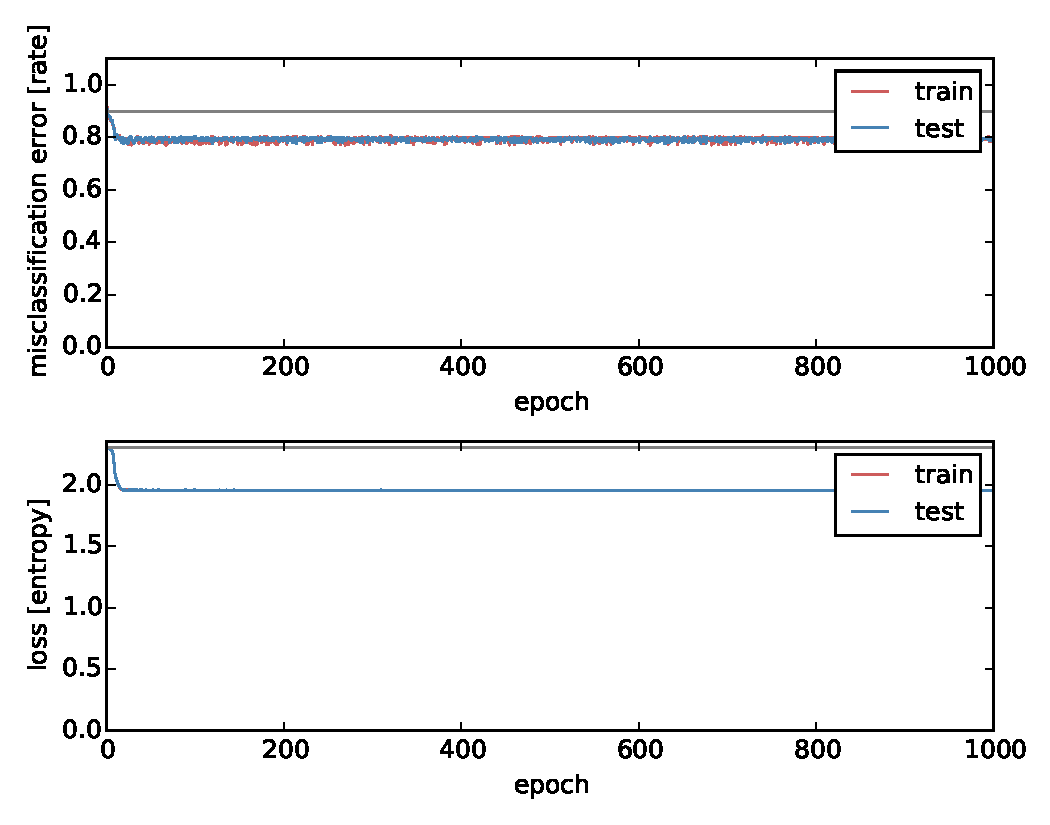
\includegraphics[scale=0.60]{results/sutskever-network-normal-01-rmsgraves}
	\caption{Loss and misclassification rate as a function of the number of epochs on the full Sutskever network.}
	\label{fig:results:sutskever:network-01}
\end{figure}
\begin{figure}[H]
        \vspace{-0.5cm}
        \centering
        \begin{subfigure}[b]{0.49\textwidth}
                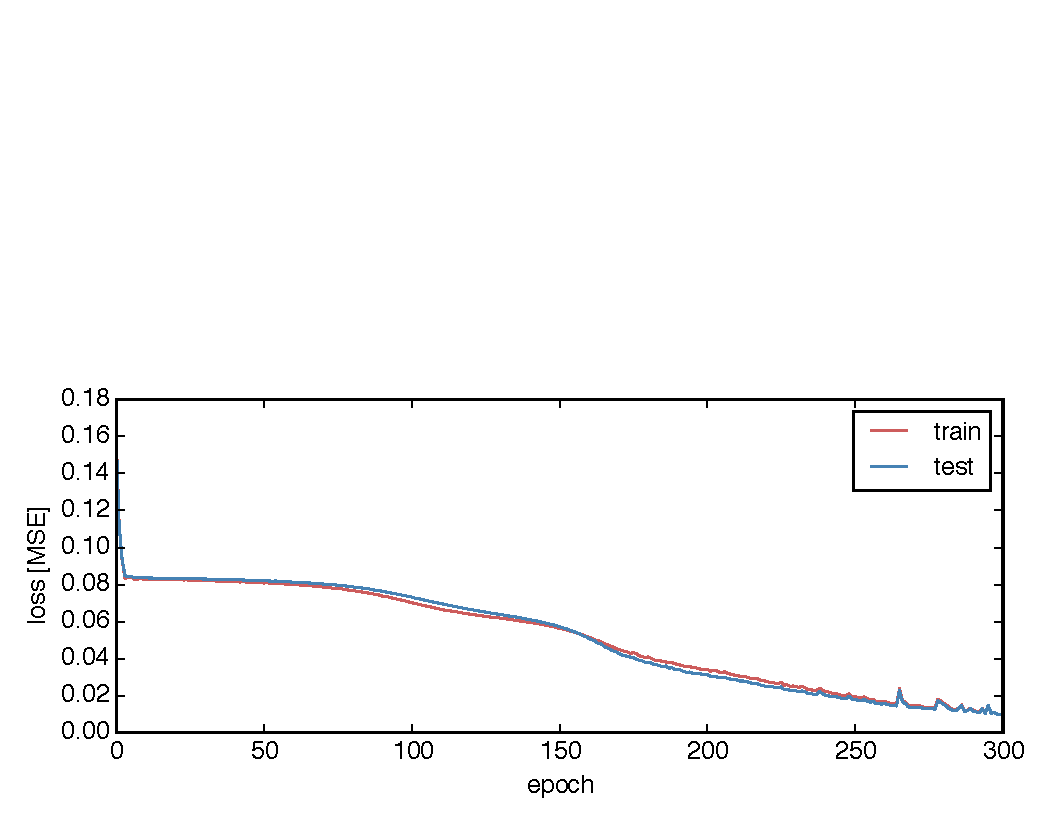
\includegraphics[scale=0.60]{results/sutskever-encoder-normal-01-rmsgraves}
                \caption{Encoder}
        \end{subfigure}
        \begin{subfigure}[b]{0.49\textwidth}
                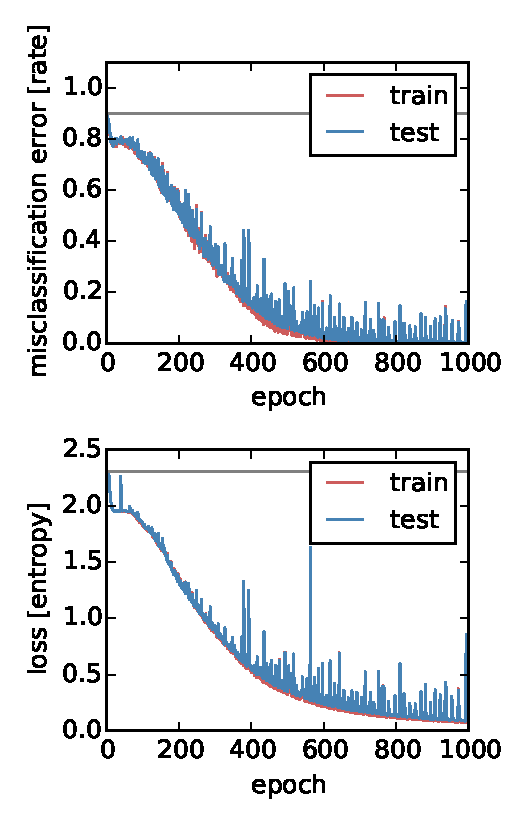
\includegraphics[scale=0.60]{results/sutskever-decoder-normal-01-rmsgraves}
                \caption{Decoder}
        \end{subfigure}
        \caption{Loss and misclassification rate as a function of the number of epochs.}
        \label{fig:results:sutskever:decoder-encoder-01}
\end{figure}

There is a lot of spikes in the encoder and decoder loss curves (Figure \ref{fig:results:sutskever:decoder-encoder-01}) these could probably have been avoided by choosing a smaller \textit{clip} value. Likewise it is entirely possible that some other hyperparameter choices could have caused the full network to converge probably. To investigate that possibility a grid search over the hyperparameters was performed.

\begin{table}[h]
\centering
\begin{tabular}{r|c}
	parameter & value(s) \\ \hline
	learning rate ($\eta$) & [0.0001, 0.001, 0.01, 0.1, 0.2] \\
	momentum ($m$) & [0, 0.2, 0.9] \\
	decay ($\gamma$) & [0.9, 0.95] \\
	weight initialization & $\mathcal{N}(0, 0.1^2)$ \\
	clipping strategy & Euclidean \\
	clipping value & [1, 5, 10, 50]
\end{tabular}
\caption{Tried parameter values for solving the \textit{full network copy} problem.}
\label{table:resutls:sutskever:gridsearch-range}
\end{table}
\begin{table}[h]
\vspace{-0.5cm}
\centering
\begin{tabular}{r|c|c}
	parameter & best & worst  \\ \hline
	learning rate ($\eta$) & 0.01 & 0.1 \\
	momentum ($m$) & 0.9 & 0 \\
	decay ($\gamma$) & 0.9 & 0.9 \\
	weight initialization & $\mathcal{N}(0, 0.1^2)$ & $\mathcal{N}(0, 0.1^2)$ \\
	clipping strategy & Euclidean & Euclidean \\
	clipping value & 5 & 10
\end{tabular}
\caption{Best and worst choose for hyperparameters, given the grid search in Table \ref{table:resutls:sutskever:gridsearch-range}.}
\end{table}

While there are good and bad choices none of them makes the full network converge, as seen in Figure \ref{fig:results:sutskever:gridsearch-clip} and \ref{fig:results:sutskever:gridsearch-momentum}.
\begin{figure}[h]
	\centering
	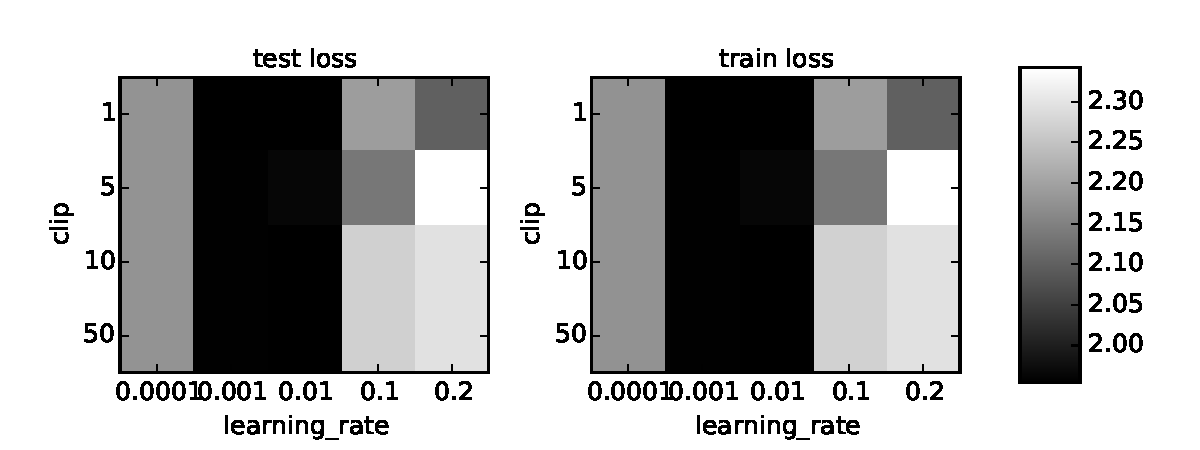
\includegraphics[scale=0.60]{results/sutskever-gridsearch-clip}
	\caption{Grid search on learning rate and clip, other parameter variations are meaned out.}
	\label{fig:results:sutskever:gridsearch-clip}
\end{figure}
\begin{figure}[H]
	\centering
	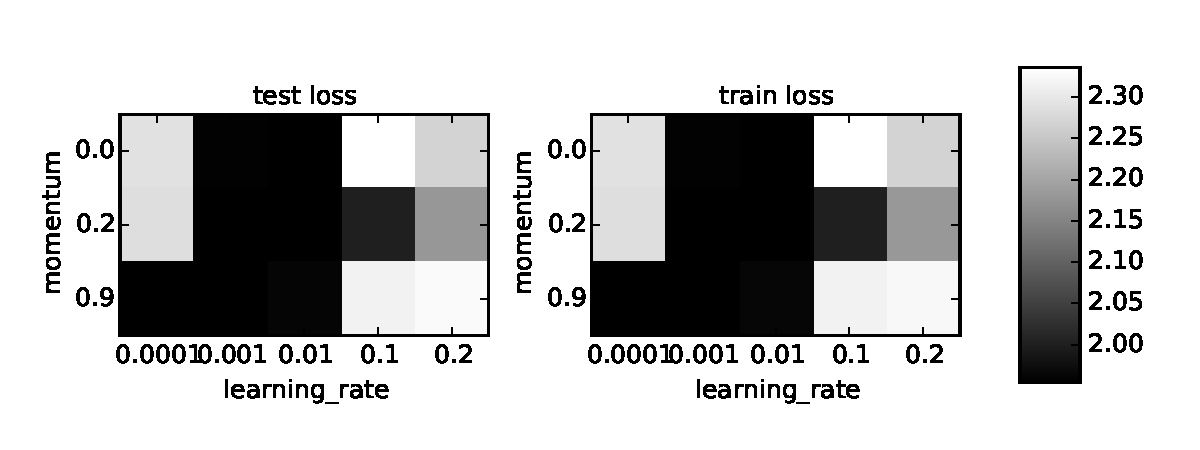
\includegraphics[scale=0.60]{results/sutskever-gridsearch-momentum}
	\caption{Grid search on learning rate and momentum, other parameters variations are meaned out.}
	\label{fig:results:sutskever:gridsearch-momentum}
\end{figure}

The encoder and decoder themselves can converge and hyperparameter optimization of the full network doesn't work. All this suggests that it is the combination of the many layers and the smaller standard deviance that causes the problem.

\subsection{Vanishing gradient}
It is not unusual that deep networks and small initial weights causes problems. This is because of the vanishing gradient problem. This is particular a problem in recurrent neural networks, because the iteration over the sequence actually causes the network to be much deeper than it appears to be. Using LSTM units solves this to some extent, however having many layers is still an issue. This is best seen by just considering a simple feed forward neural network with many layers and following the $\delta$ calculations.

Because the last layer is a softmax and one can expect and uniform distribution as the initial distribution and the target is often zero, $\delta_{L+1}$ can be approximated as $\frac{1}{10}$ (there are 10 classes). The remaining $\delta$ values are then calculated as:
\begin{equation}
\delta_{h_\ell} = \theta'(a_{h_\ell}) \sum_{h_{\ell+1} = 1}^{H_{\ell+1}} \delta_{h_{\ell+1}} w_{h_\ell, h_{\ell+1}}
\end{equation}

The maximum value of $\theta'(\cdot)$ when $\theta$ is the sigmoid function is approximately $0.23$, and one shouldn't expect more than $0.1$ from the weights given the initialization. One then gets:
\begin{equation}
\delta_{h_L} \approx 0.23 \sum_{h_{\ell+1} = 1}^{H_{\ell+1}} \frac{1}{10} \cdot 0.1 \lesssim \delta_{h_{L+1}} \approx \frac{1}{10}
\end{equation}

The $\delta_{h_\ell}$ will thus decrease for each layer causing the gradients for the bottom layers to be near zero.

Note that because the size of $\delta_{h_\ell}$ depends on $H_{\ell+1}$, one could use different standard deviance values depending on the $H_{\ell+1}$ value for each layer, such that the $\delta_{h_\ell}$ value is in a reasonable range. This was attempted and didn't work, though more experiments could have been done. Another solution is to use rectified linear unit (ReLU) as the activation function, which as been shown not to suffer from the vanishing gradient problem. Due to the lack of time this was not attempted.

